\documentclass[../main.tex]{subfiles}
\graphicspath{{\subfix{../images/}}}
\begin{document}
\subsection{LRT For Simple Hypotheses}
\begin{lemma}[Neyman - Pearson]
Given a sampling $\overrightarrow{Y}\sim f_{\theta}(\overrightarrow{y})$ and 2 simple hypotheses - 
\[H_0:\theta = \theta_0,\text{ and } H_1:\theta = \theta_1\]
The likelihood ratio test with the rejection area
\[\Omega_1:=\{\overrightarrow{y}\mid\lambda(\overrightarrow{y}):=\frac{f_{\theta_1}(\overrightarrow{y})}{f_{\theta_0}(\overrightarrow{y})}\geq C\}\]
Is a maximal power test at significance level $\alpha = \mathbb{P}_{\theta}(\lambda(\overrightarrow{Y})\geq C)$
\end{lemma}
\begin{proof}
We will prove for continuous random variables, but it is extendable to discrete ones. It now makes sense to calculate the power of the LRT. 
\[\pi:=\mathbb{P}_{\theta_1}(\lambda(\overrightarrow{Y})\geq C) = \mathbb{P}(\overrightarrow{Y}\in\Omega_1) = \int_{\Omega_1} f_{\theta_1}(\overrightarrow{y})d\overrightarrow{y}\]
Now assume we have another test with significance $\alpha'\leq \alpha$ and with power $\pi'$ and rejection region $\Omega_1'$. Again we have
\[\pi':=\mathbb{P}_{\theta_1}(\lambda(\overrightarrow{Y})\geq C) = \mathbb{P}(\overrightarrow{Y}\in\Omega_1') = \int_{\Omega_1'} f_{\theta_1}(\overrightarrow{y})d\overrightarrow{y}\]
Also
\[\alpha':=\mathbb{P}_{\theta_0}(\overrightarrow{Y}\in\Omega_1') = \int_{\Omega_1'} f_{\theta_0}(\overrightarrow{y})d\overrightarrow{y}\]
We now want to show that $\pi\geq \pi'$:
\[\pi-\pi'=\int_{\Omega_1} f_{\theta_1}(\overrightarrow{y})d\overrightarrow{y} - \int_{\Omega_1'} f_{\theta_1}(\overrightarrow{y})d\overrightarrow{y} =\]\[= \int_{\Omega_0'\cap\Omega_1} f_{\theta_1}(\overrightarrow{y})d\overrightarrow{y} + \int_{\Omega_1'\cap\Omega_1} f_{\theta_1}(\overrightarrow{y})d\overrightarrow{y} - \int_{\Omega_1'\cap\Omega_1} f_{\theta_1}(\overrightarrow{y})d\overrightarrow{y} - \int_{\Omega_1'\cap\Omega_0} f_{\theta_1}(\overrightarrow{y})d\overrightarrow{y}=\]\[=\int_{\Omega_1\cap\Omega_0'} f_{\theta_1}(\overrightarrow{y})d\overrightarrow{y} - \int_{\Omega_1'\cap\Omega_0} f_{\theta_1}(\overrightarrow{y})d\overrightarrow{y}\]
Using the definition of $\Omega_1$ we can now know that this tells us that
\[\pi-\pi'\geq \int_{\Omega_1\cap\Omega_0} Cf_{\theta_0}(\overrightarrow{y})d\overrightarrow{y} - \int_{\Omega_1'\cap\Omega_0} Cf_{\theta_0}(\overrightarrow{y})d\overrightarrow{y} = C\cdot\left(\int_{\Omega_1} f_{\theta_0}(\overrightarrow{y})d\overrightarrow{y}- \int_{\Omega_1'} f_{\theta_0}(\overrightarrow{y})d\overrightarrow{y}\right) = \]\[=C\cdot(\alpha-\alpha')\geq 0\]
Meaning we have that the power of LRT test is always greater or equal to the power of any other test, and we are done. 
\end{proof}
\begin{example}
You are in a bar europe and you meet another person who you know is either french or british. You know that certain nationalities drink certain drinks in different probabilities. You can look at what drink they have, and you want to create a test that will allow you to know the nationality of this person. Assuming you take significance $\alpha=0.25$ and your hypotheses are
\[H_0: \text{ "They are french"}, \text{ and }H_0: \text{ "They are british"}\]
The table of drink per nation is the following
\begin{center}
    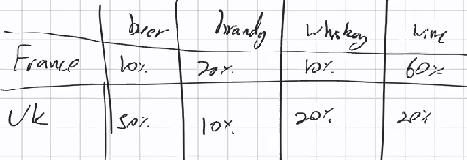
\includegraphics{images/Lecture 12 Table.png}
\end{center}
Notice that we see what type of drinks the person drinks and we want to decide what nationality they are. Meaning when we see a certain drink we should already have a deterministic guess for nationality. In order to have the significance that was stated above the possible rejection regions are
\[\{\text{Beer}\}, \{\text{Brandy}\}, \{\text{Whiskey}\}\{\text{Brandy, Beer}\}\]
The powers are
\[\pi_{\{\text{Brandy}\}} = 0.1\text{, and }\pi_{\{\text{Brandy, Beer}\}} = 0.7\]
This gives us a test for nationality based on what the persons drinks. Now we can consider the LRT. This is
\[\lambda(\overrightarrow{y}) = \frac{\mathbb{P}_{\text{UK}}(\overrightarrow{y})}{\mathbb{P}_{\text{France}}(\overrightarrow{y})}\]
This gives us the following table of values of $\lambda$
\begin{center}
    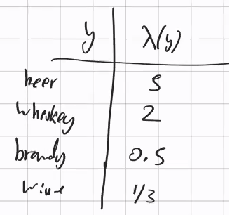
\includegraphics{images/Lambda Values Table.png}
\end{center}
We can now examine how the powers change in the following table
\begin{center}
    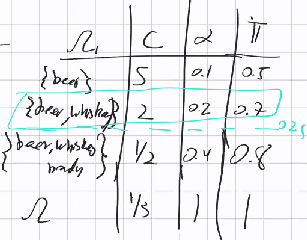
\includegraphics{images/Lecture 12 Total Table.png}
\end{center}
\end{example}
As we can see we have a discrete distribution and we can't find the specific significance we want. In continuous distributions though we can find the significance we want and so given a significance value $\alpha$ we need to rescue our C to get the test that we want for LRT. Now we can consider "composite" hypotheses (where there can be various different values of $\theta$ we can get). 
\newpage
\subsection{Composite Hypotheses}
Until now we have dealt with singletons for hypotheses, but in the real world usually the hypotheses are more than just a singleton and so we will need to give new definitions.
\begin{definition}
Given composite hypotheses we define the power function
\[\pi(\theta):=\mathbb{P}_{\theta}(\text{"reject } H_0\text{"}) = \mathbb{P}_{\theta}(\overrightarrow{Y}\in\Omega_1)\]
\end{definition}
\begin{definition}
The significance of a test on composite hypotheses is
\[\alpha:=\sup_{\theta\in\Theta_0}\mathbb{P}_{\theta}(\overrightarrow{Y}\in\Omega_1)\]
\end{definition}
\begin{definition}
If $T(\overrightarrow{Y}) = t_{\text{obs}}$ then the p-value as
\[p_{\text{value}}:=\sup_{\theta\in\Theta_0}\mathbb{P}_{\theta_0}(T(\overrightarrow{Y})\geq t_{\text{obs}})\]
\end{definition}
\end{document}